% For the listing caption reference
%! Suppress = UnresolvedReference

% To ignore word count of agent hyperparameters
%TC:group longtable 0 0

\chapter{Implementing a flexible resource allocation environment and agents}\label{ch:implementation-of-the-solution}
In order to implement a solution from chapter~\ref{ch:proposed-solution}, an MEC network environment
must be simulated due to the impractically of setting up such a network and in order to train the agents offline as
proposed in section~\ref{sec:proposed-agents}. This chapter splits the implementation into three sections: the
environment simulation (section~\ref{sec:simulating-edge-cloud-computing-services}), server auction and resource
allocation agents (section~\ref{sec:implementing-auction-and-resource-allocation-agents}) and training of agents
(section~\ref{sec:training-agents}).

The implementation discussed below as written in Python and available to download from
Github~\footnote{\url{https://github.com/stringtheorys/Online-Flexible-Resource-Allocation}}. The reason for the use of
python is number of modules available for reinforcement learning and the speed of development.

\section{Simulating edge cloud computing services}\label{sec:simulating-edge-cloud-computing-services}
While the aim of the environment is the simulate accurately MEC servers, the implementation of the environment must
allow agents to train on interact and training on the environment efficiently. Therefore it has been implemented
as an OpenAI gym~\citep{openaigym}, the de facto standard for implementing reinforcement learning environment for
researchers. However the standard specification must be modified due to the problem being multi-agent and multi-step.

An example for running the environment is in listing~\ref{lst:example_flexible_resource_env}. There are three
sections to the code: the first is the construct an environment using the constructor, where the environment settings
are passed that determines the number of servers, tasks and their attributes. These attributes are determined using
uniform random numbers between a maximum and minimum values that are synthetically generated for each variable. The
second step is to create the environment using the reset function returning the new environment state. The environment
state contains a task if one needs to be auctioned and a dictionary of server to their current task state. Using these
states, each server can generate actions either using the auction agent or resource allocation agent depending if a task
needs auctioning. The final part is to take a step using the server actions that returns an updated server state, the
rewards for the actions, if the environment is finished and an extra information from the steps taken. The rewards is a
dictionary of each of servers with either the winning price for the auctioned task or a list of tasks that have
finished either because they ran out of time or completed the task early, depending on the step taken.

\begin{lstlisting}[language=Python, frame=single, caption={Example code for running the environment}, captionpos=b, label={lst:example_flexible_resource_env}]
# Load the environment with a setting
env = OnlineFlexibleResourceAllocationEnv('settings.env')

# Generate the environment state
server_state = env.reset()

for _ in range(1000):
    # Generate actions
    if server_state.auction_task:
        actions = {
            server: auction_agent.bid(state)
            for server, state in server_state
        }
    else:
        actions = {
            server: resource_allocation_agent.weights(state)
            for server, state in server_state
        }

    # Take environment step
    server_state, reward, done, info = env.step(actions)

    # If the environment is finished then reset it
    if done:
        server_state = env.reset()
\end{lstlisting}

\subsection{Weighted server resource allocation}\label{subsec:weighted-server-resource-allocation}
A particular complication of the environment is to distribute server resources due to the fact that the resource
allocation agents provide a resource weighting rather than the actually task resource usage. Because of this, a novel
algorithm was implemented to convert the weighting to actual resources for each task.

To allocate the computational resources is relatively simple compared to allocating resources for both storage and
bandwidth. For computational resources, the algorithm checks first if the weighted resources is greater than the
quantity required for the task to finish the compute stage of a task. If this is true then a resources needed for the
task to complete the compute stage are allocated. However, this also means that the weight resources available for each
task is increased due to a task not using all of the resources it could. This type of checking is repeated till no task
can be finished with its weighted resource within this time step. For the remaining task, they are just allocated their
weighted compute resources.

For allocating storage and bandwidth, this is more difficult is due to the fact that when the server is still
loading the task, the server is allocating both storage and bandwidth resources while also allocating bandwidth
resources to tasks sending results back to users. Because of this, a tension exists between allocating bandwidth and
storage resources for all of the tasks fairly. Algorithm was therefore chosen to gives priority when allocating
resources to the tasks sending results as these tasks are more likely to be finished and aims to not penalise the
server for not completing the task within the deadline.

To allocate resources, a similar function to used to the one for allocating compute resources. First a check if done
using the weighted bandwidth resources to see if any task sending results will be finished with the resources.
This process is also repeated for the tasks loaded onto a server with the additional check that there is enough
available storage for the new data to be added. For any remaining task, this process is repeated till all of the
available resources are allocated in the time step. As a results, using this algorithm, the converting between
weightings to resources allowing for allocating of almost all of the server's resources with no resources unused.

\section{Implementing Auction and resource allocation agents}\label{sec:implementing-auction-and-resource-allocation-agents}
To implement auction and resource allocation agents, generic abstract classes for both were implemented with a bid
function for the auction agent and a weighting function for the resource weighting agent. The bid had arguments for the
task being auctioned, the server with its currently allocated tasks and current time step. These attribute were used by
the reinforcement learning policies explained in subsection~\ref{subsec:implementing-auction-and-resource-allocation-agents}
to calculate the auction bid price. For the weighting function in the resource weighting agent, the function took a
server and a list of the server's currently allocated tasks along with the current time step. Using these attributes,
agents can return a dictionary of task weighting.

A range of different reinforcement learning techniques have been implemented, outlined in
Table~\ref{tab:reinforcement_learning_algorithms}, in order to explore the different options that a server would have
available to learn its policies.

\subsection{Implementing reinforcement learning policies}\label{subsec:implementing-auction-and-resource-allocation-agents}
The policies outlined in table~\ref{tab:reinforcement_learning_algorithms} were implemented using
tensorflow~\citep{tensorflow2015-whitepaper}, a python module developed by Google
that provides programmers the ability to construct neural network, backpropagation with custom loss function and more.
For each of the algorithms, an abstract class was implemented with a function for training and saving of the agent
neural networks. For each of these algorithms, a task pricing and resource weighting class was implemented that are
subclasses for the abstract algorithm class.

Both deep Q networks and policy gradient algorithm are based on the Q function (explained in
section~\ref{sec:reinforcement-learning})) which tries to approximate the reward at the next time step. To do
this requires a reward function and a next observation to compare to in order to train these agents. The agent's
reward function and agent training observations are detailed in subsection~\ref{subsec:agent-rewards-functions}
and~\ref{subsec:agent-training-observations}.

\begin{table}
    \centering
    \begin{tabular}{|p{5cm}|p{10cm}|} \hline
        Policy Type & Explanation \\ \hline
        Dqn~\citep{mnih2015humanlevel} & A standard deep Q learning agent that discretizes the action space with a
            target neural network and experience replay buffer. \\ \hline
        Double Dueling DQN~\citep{doubledqn, duelingdqn} & A combination of two heuristics for the standard deep Q
            learning agents that uses a modified td target function and a modified networks that separates state value
            and action advantage which can recombined at the end. \\ \hline
        Categorical Dqn~\citep{distributional_dqn} & Standard deep Q learning agents return a scalar value
            (representing the q value) for each action. Instead this outputs a probability distribution over action
            values that is believed to be helpful due to the stochastic nature from the problem (from the agents
            perspective). \\ \hline
        Deep deterministic policy gradient~\citep{ddpg} & As the action space is continuous, DDPG allows for
            investigation of the difference between continuous and discrete action spaces of the DQN agents. As policy
            gradient can be more effective at learning a policy where the reward function is too complex for DQN to
            model this may give the algorithm another advantage. \\ \hline
        Twin delay DDPG~\citep{td3} & Like the Double Dueling DQN agents, TD3 includes a couple new heuristics for the
            DDPG algorithm. A critic twin is used to prevent the actor network from tricking the critic network, another
            heuristic is the delaying the updates for actor network compared to the critic network.\\ \hline
        D4PG~\citep{d4pg} & Like the Categorical DQN algorithm, D4PG adds a heuristic for the critic to output a
            value distribution that allows for better approximation for environments that are stochastic in nature.
            \\ \hline
    \end{tabular}
    \caption{Table of the implemented reinforcement learning algorithms}
    \label{tab:reinforcement_learning_algorithms}
\end{table}

A particular problem that this project encounter was with using recurrent neural network as inputs. This is as the
number of inputs is not fixed meaning that during training, using a minibatch was not possible as most of the inputs
all had different input lengths and tensorflow requires all inputs to have a known, fixed length. Originally this was
sidestepped by calculating the loss for each input individually then finding the mean loss and gradient to update the
networks with. However this was found to be computationally impractical making the method impossible to run agents to
long enough. Because of this, a solution was found by padding all of the inputs to have the same size using the
tensorflow preprocessing module with the sequence.pad\_sequence function. As a result, training became ~10x faster
making large scale testing practical.

\subsection{Agent rewards functions}\label{subsec:agent-rewards-functions}
As explained in the background review for reinforcement learning (section~\ref{sec:reinforcement-learning}),
the Q values is the estimated discounted reward in the future for an action given a particular state. Therefore the
rewards that an agent receives for taking an action is extremely important to enable the agent to learn a predictable
reward function. This problem of complex reward functions are a known problem for DQN agent to deal with~\citep{atari}m
policy gradients can deal with this better due its ability directly learning the action policy~\citep{Sutton1998}.

For the auction, the reward is based on the winning price of the task which is award for the winning action. If the
task fails, the reward is instead multiplied by a negative constant in order to discourage the auction agent from
bidding on tasks that it wouldn't be able to complete. This reward is awarded at the time step of the auction instead of
when the task fails or is completed as this makes the function harder to learn as the auction agent has no control or
observations over the resource allocation for a task. \\
As the price of zero is treated as a non-bid in the auction, the agent gets a reward of zero in order to not
penalise the agent. But if the agent does bid on a task however doesn't win, the agent's reward is -0.05 as a way of
encouraging the agent to change there bid but not enough to force it to do so.

For resource allocation, the reward function is much simpler than the auction agent's reward function, as it only needs
to consider the task being weighted at the time and rewards from other tasks allocated at the same time step. This is
as a task must consider its actions in conjunction with the resource requirements of other allocated tasks. \\
For successfully finishing a task, the reward is 1 while the reward for if the task has failed is -1.5. This makes
failing a task more costly than completing a task. But when a task's action is not under consideration, this reward is
multiplied by 0.4 as while this rewards impact the task, their value is not as impactful as the reward for the action
on a particular task. These rewards don't consider the price payed for the task instead valuing each task equally with
the aim of forcing the task allocate resources to finish all tasks not just the valuable ones. Using this information,
the reward function is simply the sums the rewards of the finished tasks in the next time step.

\subsection{Agent training observations}\label{subsec:agent-training-observations}
As the agent acts in the environment, the observations that the agent views are stored in an experience replay buffer
which allows the agents to train from previous observations. However this is a problem for agent due to the separate
agents acting with only during its particular action step. This is outlined in figure~\ref{fig:environment-observations},
where an agents next observation is often after subsequent actions by the opposite agent.

\begin{figure}
    \centering
    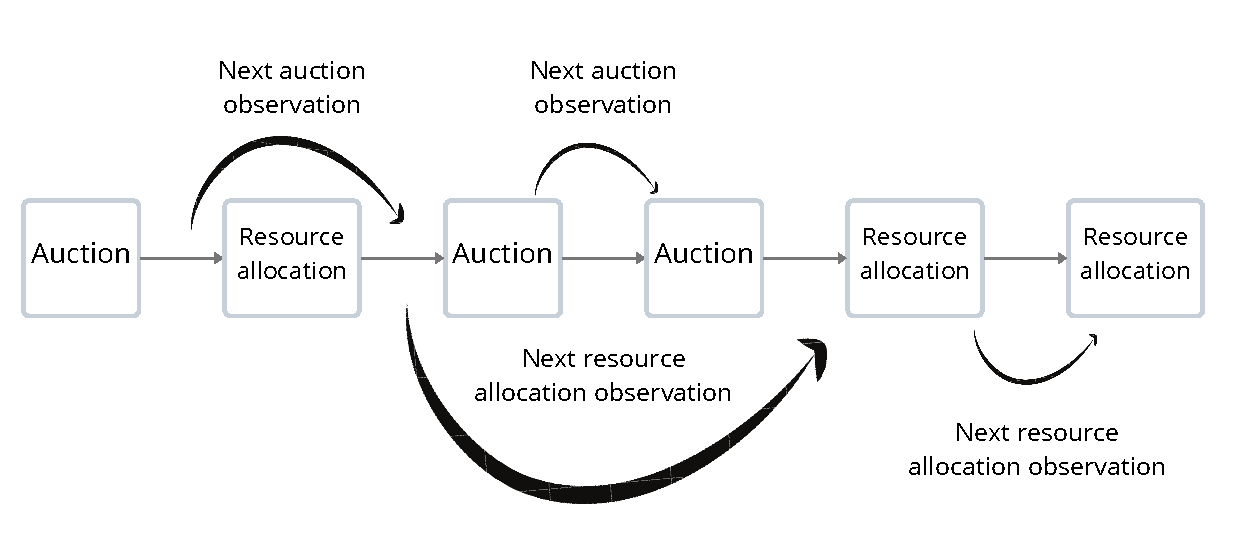
\includegraphics[width=14cm]{figures/3_implementation_figs/env_server_agents_observations.pdf}
    \caption{Environment server agents observations}
    \label{fig:environment-observations}
\end{figure}

For the resource allocation agent, a trick is implemented such that the next observation for the agent is not the
actual next resource allocation observation as shown in figure~\ref{fig:environment-observations} but a generated
observation from the resulting server state due to agent's actions. This is identical to the last case in the figure
where no auction occurs between resource allocation steps. Because of this, the resource allocation Q value is able to
approximate the reward for the results state of its actions directly making it appear to the agent during training that
there is no auction steps between the observations and next observations.
% Todo add number of tasks observations problems

For the auction agent, as the agent observations require an auction task to select an action (the task bidding price).
A trick like the one implemented for the resource allocation agent can't be to implement. Therefore during training,
each server's last observation is recorded, such that when the next auction occurs, this new task observation can be
used as the server's next observation in training. This is a suboptimal solution for the agent as the next observation
has an unknown number of resource allocation steps resulting in changes to the current allocated tasks.
A possible solution that has not been implement in this project is n step prediction~\citep{multi-step-dqn}. Where the
agent doesn't predict the Q value of the next environment, but the value in n steps time. This is believed to possible
help reduce the amount of randomness in the server's observations and improve bidding performance.

\section{Training agents}\label{sec:training-agents}
The first section of this chapter allowed for the simulating MEC servers
(section~\ref{sec:simulating-edge-cloud-computing-services}) as a reinforcement learning environment. While the second
section implements auction and resource allocation agents that can interact with the porpoised environment in order
to allow for the train of agents using a range of algorithm outlined in Table~\ref{tab:reinforcement_learning_algorithms}.

Neural networks, the bases of the reinforcement learning agents implemented, often require huge amounts of data and
high spec GPUs to run efficiently. Because of this, Iridis 5, University of Southampton supercomputer was utilised with
GTX1050 GPUs to train these agents for long periods of time and on mass. During training, for each episode a random
environment was generated from a list of possible settings in which the agents would be allocated to random servers. The
environment was run till the end, with the agent observation being added to their replay buffers after each actions
that were chosen epsilon greedily.

After every 5 episodes, the agents would be evaluated using a set of environment that were pre-generated and
saved at the beginning of training. This allows the same environments over training in order to have a constant metric
in order to compare the agents over time. The actions taken are recorded to be used in evaluation
(chapter~\ref{ch:evaluation-of-the-solution}) with the number of completed and failed tasks being stored about
the resource allocation agent and the winning prices being stored about the auction agents. Plus an action histograms
for each agents in order to view how agents bid and weightings are distributed.

\subsection{Agent training hyperparameters}\label{subsec:agent-training-hyperparameters}
During training there are a range of hyperparameters for each agent, table~\ref{tab:agent_hyperparameters} provides
an explanation of value for all of the hyperparameters used in the project.

\begin{longtable}{|p{2cm}|p{3.5cm}|p{2.5cm}|p{6cm}|} \hline
    \textbf{Agent} & \textbf{Properties name} & \textbf{Value} & \textbf{Explanation} \\ \hline
        RL Agent & batch\_size & 32 & The number of trajectories from the experience replay buffer that are used each
            time to train an agent. \\ \hline
        RL Agent & error\_loss\_fn & tf.losses. huber\_loss & The loss function for calculating the error that similar
            the mean squared loss exact has a smaller gradient. \\ \hline
        RL Agent & initial\_training replay\_size & 5000 & The number of trajectories in the experience replay buffer
            required before the agent begins training. \\ \hline
        RL Agent & training\_freq & 2 & For every trajectory added to the experience replay buffer, for each 2, the
            agent tries to be trained. \\ \hline
        RL Agent & discount\_factor & 0.9 & Within the Q learning function (equation~\eqref{eq:q_learning}), the
            discount factor determines how important the rewards in the future impact the Q value. \\ \hline
        RL Agent & replay\_buffer length & 25000 & The length of the circular experience replay buffer. \\ \hline
        RL Agent & save\_frequency & 25000 & The agent networks are saved after 25000 time that agent has been trained
            \\ \hline
        RL Agent & training\_loss log\_freq & 250 & Tensorboard allows for data to be saved using training, after every
            the agent has been trained 250 time, the agents loss is logged for future analysis. \\ \hline
        Task Pricing RL Agent & reward\_scaling & 1 & \\ \hline
        Task Pricing RL Agent & failed\_auction reward & -0.05 & The reward for when the agent bids on a task but fails
            to win the auctioned task. \\ \hline
        Task Pricing RL Agent & failed\_multiplier & -1.5 & A multiplier applied to the winning price is the task fails
            to be computed within its deadline. \\ \hline
        Resource weighting RL Agent & other\_task\_discount & 0.4 & The multiplier to tasks not under consideration for
            a weighting action. \\ \hline
        Resource weighting RL Agent & success\_reward & 1 & The reward when the agent successfully completes a task
            \\ \hline
        Resource weighting RL Agent & failed\_reward & -1.5 & The reward when the agent fails to complete a task within
            its deadline. \\ \hline
        Dqn Agent & target\_update\_tau & 1.0 & The update tau value for use in the target update frequency. \\ \hline
        Dqn Agent & target\_update\_freq & 2500 & The target network in the DQN agent is updated after the agent
            has been updated 2500 times. \\ \hline
        Dqn Agent & initial\_epsilon & 1 & The initial exploration factor during training \\ \hline
        Dqn Agent & final\_epsilon & 0.1 & The final exploration factor during training \\ \hline
        Dqn Agent & epsilon\_steps & 10000 & The number of training step for linear exploration to move between the
            initial\_epsilon and the final\_epsilon factor. \\ \hline
        Dueling Dqn Agent & double\_loss & True & If to use the double dqn loss function \\ \hline
        Categorical Dqn Agent & max\_value & -20.0 & The maximum value for the value distribution \\ \hline
        Categorical Dqn Agent & min\_value & 25.0 & The minimum value for the value distribution \\ \hline
        Categorical Dqn Agent & num\_atoms & 21 & The number of atoms for each actions. \\ \hline
        Ddpg Agent & actor\_learning\_rate & 0.0001 & The learning rate for the optimiser for the actor network. \\ \hline
        Ddpg Agent & critic\_learning\_rate & 0.0005 & The learning rate for the optimiser for the critic network. \\ \hline
        Ddpg Agent & initial\_epsilon\_std & 0.8 & The initial exploration standard deviation of the normal distribution
            used  during training \\ \hline
        Ddpg Agent & final\_epsilon\_std & 0.05 & The final exploration standard deviation of the normal distribution
            used  during training \\ \hline
        Ddpg Agent & actor\_target update\_freq & 3000 & The actor target network update frequency \\ \hline
        Ddpg Agent & critic\_target update\_freq & 1500 & The critic target network update frequency \\ \hline
        Ddpg Agent & upper\_action bound & 30.0 & The upper action bound for the actor network \\ \hline
        Task pricing Ddpg Agent & min\_value & -100.0 & The minimum value for the critic network to estimate for an
            action \\ \hline
        Task pricing Ddpg Agent & max\_value & 100.0 & The maximum value for the critic network to estimate for an
            action\\ \hline
        Resource allocation Ddpg Agent & min\_value & -20 & The minimum value for the critic network to estimate for an
            action \\ \hline
        Resource allocation Ddpg Agent & max\_value & 15 & The maximum value for the critic network to estimate for an
            action\\ \hline
        TD3 Agent & actor\_update\_freq & 3 & The actor network update frequency for each critic network update. \\ \hline
    \caption{Agent hyperparameters}
    \label{tab:agent_hyperparameters}
\end{longtable}


